%% bare_conf.tex
%% V1.4b
%% 2015/08/26
%% by Michael Shell
%% See:
%% http://www.michaelshell.org/
%% for current contact information.
%%
%% This is a skeleton file demonstrating the use of IEEEtran.cls
%% (requires IEEEtran.cls version 1.8b or later) with an IEEE
%% conference paper.
%%
%% Support sites:
%% http://www.michaelshell.org/tex/ieeetran/
%% http://www.ctan.org/pkg/ieeetran
%% and
%% http://www.ieee.org/

%%*************************************************************************
%% Legal Notice:
%% This code is offered as-is without any warranty either expressed or
%% implied; without even the implied warranty of MERCHANTABILITY or
%% FITNESS FOR A PARTICULAR PURPOSE! 
%% User assumes all risk.
%% In no event shall the IEEE or any contributor to this code be liable for
%% any damages or losses, including, but not limited to, incidental,
%% consequential, or any other damages, resulting from the use or misuse
%% of any information contained here.
%%
%% All comments are the opinions of their respective authors and are not
%% necessarily endorsed by the IEEE.
%%
%% This work is distributed under the LaTeX Project Public License (LPPL)
%% ( http://www.latex-project.org/ ) version 1.3, and may be freely used,
%% distributed and modified. A copy of the LPPL, version 1.3, is included
%% in the base LaTeX documentation of all distributions of LaTeX released
%% 2003/12/01 or later.
%% Retain all contribution notices and credits.
%% ** Modified files should be clearly indicated as such, including  **
%% ** renaming them and changing author support contact information. **
%%*************************************************************************


% *** Authors should verify (and, if needed, correct) their LaTeX system  ***
% *** with the testflow diagnostic prior to trusting their LaTeX platform ***
% *** with production work. The IEEE's font choices and paper sizes can   ***
% *** trigger bugs that do not appear when using other class files.       ***                          ***
% The testflow support page is at:
% http://www.michaelshell.org/tex/testflow/



\documentclass[conference]{IEEEtran}
\usepackage{cite}
\usepackage{graphicx}
\usepackage{hyperref}
\usepackage{float}

% Some Computer Society conferences also require the compsoc mode option,
% but others use the standard conference format.
%
% If IEEEtran.cls has not been installed into the LaTeX system files,
% manually specify the path to it like:
% \documentclass[conference]{../sty/IEEEtran}





% Some very useful LaTeX packages include:
% (uncomment the ones you want to load)


% *** MISC UTILITY PACKAGES ***
%
%\usepackage{ifpdf}
% Heiko Oberdiek's ifpdf.sty is very useful if you need conditional
% compilation based on whether the output is pdf or dvi.
% usage:
% \ifpdf
%   % pdf code
% \else
%   % dvi code
% \fi
% The latest version of ifpdf.sty can be obtained from:
% http://www.ctan.org/pkg/ifpdf
% Also, note that IEEEtran.cls V1.7 and later provides a builtin
% \ifCLASSINFOpdf conditional that works the same way.
% When switching from latex to pdflatex and vice-versa, the compiler may
% have to be run twice to clear warning/error messages.






% *** CITATION PACKAGES ***
%
%\usepackage{cite}
% cite.sty was written by Donald Arseneau
% V1.6 and later of IEEEtran pre-defines the format of the cite.sty package
% \cite{} output to follow that of the IEEE. Loading the cite package will
% result in citation numbers being automatically sorted and properly
% "compressed/ranged". e.g., [1], [9], [2], [7], [5], [6] without using
% cite.sty will become [1], [2], [5]--[7], [9] using cite.sty. cite.sty's
% \cite will automatically add leading space, if needed. Use cite.sty's
% noadjust option (cite.sty V3.8 and later) if you want to turn this off
% such as if a citation ever needs to be enclosed in parenthesis.
% cite.sty is already installed on most LaTeX systems. Be sure and use
% version 5.0 (2009-03-20) and later if using hyperref.sty.
% The latest version can be obtained at:
% http://www.ctan.org/pkg/cite
% The documentation is contained in the cite.sty file itself.






% *** GRAPHICS RELATED PACKAGES ***
%
\ifCLASSINFOpdf
  % \usepackage[pdftex]{graphicx}
  % declare the path(s) where your graphic files are
  % \graphicspath{{../pdf/}{../jpeg/}}
  % and their extensions so you won't have to specify these with
  % every instance of \includegraphics
  % \DeclareGraphicsExtensions{.pdf,.jpeg,.png}
\else
  % or other class option (dvipsone, dvipdf, if not using dvips). graphicx
  % will default to the driver specified in the system graphics.cfg if no
  % driver is specified.
  % \usepackage[dvips]{graphicx}
  % declare the path(s) where your graphic files are
  % \graphicspath{{../eps/}}
  % and their extensions so you won't have to specify these with
  % every instance of \includegraphics
  % \DeclareGraphicsExtensions{.eps}
\fi
% graphicx was written by David Carlisle and Sebastian Rahtz. It is
% required if you want graphics, photos, etc. graphicx.sty is already
% installed on most LaTeX systems. The latest version and documentation
% can be obtained at: 
% http://www.ctan.org/pkg/graphicx
% Another good source of documentation is "Using Imported Graphics in
% LaTeX2e" by Keith Reckdahl which can be found at:
% http://www.ctan.org/pkg/epslatex
%
% latex, and pdflatex in dvi mode, support graphics in encapsulated
% postscript (.eps) format. pdflatex in pdf mode supports graphics
% in .pdf, .jpeg, .png and .mps (metapost) formats. Users should ensure
% that all non-photo figures use a vector format (.eps, .pdf, .mps) and
% not a bitmapped formats (.jpeg, .png). The IEEE frowns on bitmapped formats
% which can result in "jaggedy"/blurry rendering of lines and letters as
% well as large increases in file sizes.
%
% You can find documentation about the pdfTeX application at:
% http://www.tug.org/applications/pdftex





% *** MATH PACKAGES ***
%
%\usepackage{amsmath}
% A popular package from the American Mathematical Society that provides
% many useful and powerful commands for dealing with mathematics.
%
% Note that the amsmath package sets \interdisplaylinepenalty to 10000
% thus preventing page breaks from occurring within multiline equations. Use:
%\interdisplaylinepenalty=2500
% after loading amsmath to restore such page breaks as IEEEtran.cls normally
% does. amsmath.sty is already installed on most LaTeX systems. The latest
% version and documentation can be obtained at:
% http://www.ctan.org/pkg/amsmath





% *** SPECIALIZED LIST PACKAGES ***
%
%\usepackage{algorithmic}
% algorithmic.sty was written by Peter Williams and Rogerio Brito.
% This package provides an algorithmic environment fo describing algorithms.
% You can use the algorithmic environment in-text or within a figure
% environment to provide for a floating algorithm. Do NOT use the algorithm
% floating environment provided by algorithm.sty (by the same authors) or
% algorithm2e.sty (by Christophe Fiorio) as the IEEE does not use dedicated
% algorithm float types and packages that provide these will not provide
% correct IEEE style captions. The latest version and documentation of
% algorithmic.sty can be obtained at:
% http://www.ctan.org/pkg/algorithms
% Also of interest may be the (relatively newer and more customizable)
% algorithmicx.sty package by Szasz Janos:
% http://www.ctan.org/pkg/algorithmicx




% *** ALIGNMENT PACKAGES ***
%
%\usepackage{array}
% Frank Mittelbach's and David Carlisle's array.sty patches and improves
% the standard LaTeX2e array and tabular environments to provide better
% appearance and additional user controls. As the default LaTeX2e table
% generation code is lacking to the point of almost being broken with
% respect to the quality of the end results, all users are strongly
% advised to use an enhanced (at the very least that provided by array.sty)
% set of table tools. array.sty is already installed on most systems. The
% latest version and documentation can be obtained at:
% http://www.ctan.org/pkg/array


% IEEEtran contains the IEEEeqnarray family of commands that can be used to
% generate multiline equations as well as matrices, tables, etc., of high
% quality.




% *** SUBFIGURE PACKAGES ***
%\ifCLASSOPTIONcompsoc
%  \usepackage[caption=false,font=normalsize,labelfont=sf,textfont=sf]{subfig}
%\else
%  \usepackage[caption=false,font=footnotesize]{subfig}
%\fi
% subfig.sty, written by Steven Douglas Cochran, is the modern replacement
% for subfigure.sty, the latter of which is no longer maintained and is
% incompatible with some LaTeX packages including fixltx2e. However,
% subfig.sty requires and automatically loads Axel Sommerfeldt's caption.sty
% which will override IEEEtran.cls' handling of captions and this will result
% in non-IEEE style figure/table captions. To prevent this problem, be sure
% and invoke subfig.sty's "caption=false" package option (available since
% subfig.sty version 1.3, 2005/06/28) as this is will preserve IEEEtran.cls
% handling of captions.
% Note that the Computer Society format requires a larger sans serif font
% than the serif footnote size font used in traditional IEEE formatting
% and thus the need to invoke different subfig.sty package options depending
% on whether compsoc mode has been enabled.
%
% The latest version and documentation of subfig.sty can be obtained at:
% http://www.ctan.org/pkg/subfig




% *** FLOAT PACKAGES ***
%
%\usepackage{fixltx2e}
% fixltx2e, the successor to the earlier fix2col.sty, was written by
% Frank Mittelbach and David Carlisle. This package corrects a few problems
% in the LaTeX2e kernel, the most notable of which is that in current
% LaTeX2e releases, the ordering of single and double column floats is not
% guaranteed to be preserved. Thus, an unpatched LaTeX2e can allow a
% single column figure to be placed prior to an earlier double column
% figure.
% Be aware that LaTeX2e kernels dated 2015 and later have fixltx2e.sty's
% corrections already built into the system in which case a warning will
% be issued if an attempt is made to load fixltx2e.sty as it is no longer
% needed.
% The latest version and documentation can be found at:
% http://www.ctan.org/pkg/fixltx2e


%\usepackage{stfloats}
% stfloats.sty was written by Sigitas Tolusis. This package gives LaTeX2e
% the ability to do double column floats at the bottom of the page as well
% as the top. (e.g., "\begin{figure*}[!b]" is not normally possible in
% LaTeX2e). It also provides a command:
%\fnbelowfloat
% to enable the placement of footnotes below bottom floats (the standard
% LaTeX2e kernel puts them above bottom floats). This is an invasive package
% which rewrites many portions of the LaTeX2e float routines. It may not work
% with other packages that modify the LaTeX2e float routines. The latest
% version and documentation can be obtained at:
% http://www.ctan.org/pkg/stfloats
% Do not use the stfloats baselinefloat ability as the IEEE does not allow
% \baselineskip to stretch. Authors submitting work to the IEEE should note
% that the IEEE rarely uses double column equations and that authors should try
% to avoid such use. Do not be tempted to use the cuted.sty or midfloat.sty
% packages (also by Sigitas Tolusis) as the IEEE does not format its papers in
% such ways.
% Do not attempt to use stfloats with fixltx2e as they are incompatible.
% Instead, use Morten Hogholm'a dblfloatfix which combines the features
% of both fixltx2e and stfloats:
%
% \usepackage{dblfloatfix}
% The latest version can be found at:
% http://www.ctan.org/pkg/dblfloatfix




% *** PDF, URL AND HYPERLINK PACKAGES ***
%
%\usepackage{url}
% url.sty was written by Donald Arseneau. It provides better support for
% handling and breaking URLs. url.sty is already installed on most LaTeX
% systems. The latest version and documentation can be obtained at:
% http://www.ctan.org/pkg/url
% Basically, \url{my_url_here}.




% *** Do not adjust lengths that control margins, column widths, etc. ***
% *** Do not use packages that alter fonts (such as pslatex).         ***
% There should be no need to do such things with IEEEtran.cls V1.6 and later.
% (Unless specifically asked to do so by the journal or conference you plan
% to submit to, of course. )


% correct bad hyphenation here
\hyphenation{op-tical net-works semi-conduc-tor}
\usepackage{listings}
\usepackage{xcolor}
\usepackage{algorithm}
\usepackage{algpseudocode}
\usepackage{amsmath}

\begin{document}
%
% paper title
% Titles are generally capitalized except for words such as a, an, and, as,
% at, but, by, for, in, nor, of, on, or, the, to and up, which are usually
% not capitalized unless they are the first or last word of the title.
% Linebreaks \\ can be used within to get better formatting as desired.
% Do not put math or special symbols in the title.
\title{Análisis y Aplicaciones del Red-Black Tree}


% author names and affiliations
% use a multiple column layout for up to three different
% affiliations
\author{\IEEEauthorblockN{Galindo Bendezu, Marco Antonio}
\IEEEauthorblockA{Dept. de Computer Science\\
UTEC\\
Lima, Perú\\
%Atlanta, Georgia 30332--0250\\
marco.galindo.b@utec.edu.pe}
\and
\IEEEauthorblockN{Alferez Vicente, Bladimir}
\IEEEauthorblockA{Dept. de Data Science\\
UTEC\\
Lima, Perú\\
bladimir.alferez@utec.edu.pe}
\and
\IEEEauthorblockN{Ildefonso Santos, Steve}
\IEEEauthorblockA{Dept. de Computer Science\\
UTEC\\
Lima, Perú\\
steve.ildefonso@utec.edu.pe}}

% conference papers do not typically use \thanks and this command
% is locked out in conference mode. If really needed, such as for
% the acknowledgment of grants, issue a \IEEEoverridecommandlockouts
% after \documentclass

% for over three affiliations, or if they all won't fit within the width
% of the page, use this alternative format:
% 
%\author{\IEEEauthorblockN{Michael Shell\IEEEauthorrefmark{1},
%Homer Simpson\IEEEauthorrefmark{2},
%James Kirk\IEEEauthorrefmark{3}, 
%Montgomery Scott\IEEEauthorrefmark{3} and
%Eldon Tyrell\IEEEauthorrefmark{4}}
%\IEEEauthorblockA{\IEEEauthorrefmark{1}School of Electrical and Computer Engineering\\
%Georgia Institute of Technology,
%Atlanta, Georgia 30332--0250\\ Email: see http://www.michaelshell.org/contact.html}
%\IEEEauthorblockA{\IEEEauthorrefmark{2}Twentieth Century Fox, Springfield, USA\\
%Email: homer@thesimpsons.com}
%\IEEEauthorblockA{\IEEEauthorrefmark{3}Starfleet Academy, San Francisco, California 96678-2391\\
%Telephone: (800) 555--1212, Fax: (888) 555--1212}
%\IEEEauthorblockA{\IEEEauthorrefmark{4}Tyrell Inc., 123 Replicant Street, Los Angeles, California 90210--4321}}




% use for special paper notices
%\IEEEspecialpapernotice{(Invited Paper)}




% make the title area
\maketitle

% As a general rule, do not put math, special symbols or citations
% in the abstract
\begin{abstract}

Los Red Black Tree son estructuras de datos que garantizan un eficiente manejo y organización de información ordenada. Basados en BST, mantienen su equilibrio a través de un sistema sencillo pero eficaz de colores (rojo y negro) asignados a cada nodo, asegurando que ninguna ruta desde la raíz hasta cualquier hoja sea significativamente más larga que otra. Este documento presenta una revisión teórica y práctica de los Red Black Tree, analiza su complejidad, y explora su rendimiento mediante evaluaciones experimentales, y destaca sus aplicaciones prácticas más relevantes.


\end{abstract}

% no keywords




% For peer review papers, you can put extra information on the cover
% page as needed:
% \ifCLASSOPTIONpeerreview
% \begin{center} \bfseries EDICS Category: 3-BBND \end{center}
% \fi
%
% For peerreview papers, this IEEEtran command inserts a page break and
% creates the second title. It will be ignored for other modes.
\IEEEpeerreviewmaketitle



% Introduccion ---------------------------------------------------
\section{Introducción}

Una de las mayores dificultades al almacenar y gestionar información es mantener los datos organizados de forma que las operaciones sean rápidas y efectivas. Por ello, surgieron diversos tipos de árboles, como los árboles 2-3, que representaron una solución inicial para asegurar un balanceo adecuado y mantener un rendimiento óptimo en las operaciones de búsqueda, inserción y eliminación \cite{baeldungRedBlack}. Tomando como referencia estas estructuras, en 1972 Rudolf Bayer introdujo los Árboles Rojo-Negro (Red-Black Trees), denominados originalmente \textit{Symmetric Binary B-Trees}, como una alternativa más eficiente basada en árboles binarios \cite{ahuja2021}.\\

Los árboles binarios de búsqueda (BST, por sus siglas en inglés) son estructuras fundamentales para organizar datos ordenados \cite{baeldungRedBlack}. Cada nodo en un BST puede tener hasta dos hijos: uno izquierdo con valores menores y otro derecho con valores mayores, lo que facilita operaciones rápidas. Sin embargo, si los datos se insertan de manera desordenada o secuencial, estos árboles pueden volverse ineficientes debido a un crecimiento excesivo en su altura, llegando incluso a degenerarse en una lista enlazada. Esto provoca que las operaciones tengan una complejidad de hasta \( O(n) \) en el peor caso, lo cual ralentiza  el rendimiento.\\

Para resolver este problema, los Red Black Trees utilizan una técnica basada en la asignación de colores (rojo o negro) a cada nodo y el cumplimiento de reglas específicas sobre estos colores. Estas reglas permiten que el árbol permanezca aproximadamente balanceado en todo momento \cite{mushiba2024redblack}, limitando su profundidad máxima a aproximadamente el doble de la mínima. Gracias a esta propiedad, las operaciones de búsqueda, inserción y eliminación se realizan en tiempo \( O(\log n) \), independientemente del orden de inserción de los elementos \cite{mushiba2024redblack}.\\

Los Red Black Trees son altamente populares por varias razones importantes \cite{morin2013ods}:

\begin{itemize}
    \item La altura máxima del árbol que almacena \( n \) elementos es \( 2 \log n \).
    \item Las operaciones de inserción y eliminación siempre toman tiempo \( O(\log n) \) en el peor caso.
    \item El número de rotaciones necesarias para equilibrar el árbol después de insertar o eliminar elementos es muy bajo, siendo una constante amortizada 
\end{itemize} 

Estas ventajas posicionan a los Red Black Trees por encima de estructuras como los skiplists, treaps y árboles scapegoat, que aunque logran tiempos similares, tienen otras limitaciones o requieren uso de técnicas probabilísticas \cite{morin2013ods}.\\

Por su eficiencia y balance garantizado, los Red Black Trees son muy usados en aplicaciones prácticas, como en la gestión de datos en la Biblioteca Estándar de Java (Java Collections Framework), diversas implementaciones de la Librería Estándar de C++ (Standard Template Library) y en el núcleo del sistema operativo Linux\cite{morin2013ods}.\\

% Fin Intro ---------------------------------------------------


% Explicación ---------------------------------------------------
\section{Fundamentos Teóricos}

Los Red Black Trees (RB Trees), como se detallo anteriormente, son un tipo de árbol binario de búsqueda auto-balanceado, utilizados para almacenar pares clave/valor ordenables. A diferencia de los \textit{radix trees}, que están optimizados para almacenar arreglos dispersos con índices enteros largos, o las tablas hash, que no mantienen el orden y dependen de una función hash bien ajustada, los RB Trees permiten escalar eficientemente almacenando claves arbitrarias manteniendo el orden de los datos \cite{linuxrbtree}.\\

Además, los RB Trees son similares a los árboles AVL, pero ofrecen un mejor rendimiento en tiempo real para inserciones y eliminaciones en el peor caso. Mientras que los árboles AVL pueden requerir múltiples rotaciones, los RB Trees realizan como máximo dos rotaciones durante una inserción y tres durante una eliminación, manteniendo un tiempo de búsqueda de \( O(\log n) \), aunque ligeramente más lento que AVL \cite{linuxrbtree}.\\

Cada nodo de un RB Tree contiene un bit adicional que representa su color (rojo o negro), el cual se utiliza para mantener el balance del árbol después de operaciones de inserción o eliminación. Las siguientes propiedades deben cumplirse \cite{jaiswal2018}\cite{cormen2001}\cite{nguyen2019}:\\

\begin{enumerate}
    \item Un RB Tree debe ser un BST.
    \item La raíz del árbol debe ser de color negro.
    \item Todos los nodos hoja (\texttt{NIL}) son negros y no contienen claves.
    \item Cada nodo es de color rojo o negro.
    \item Si un nodo es rojo, entonces ambos hijos deben ser negros. No se permiten nodos rojos consecutivos (padre e hijo).
    \item Todo nuevo nodo que se inserta se colorea inicialmente como rojo.
    \item Todo camino simple desde un nodo hasta cualquier hoja descendiente contiene la misma cantidad de nodos negros (\textit{black-height} uniforme).
    \item Los subárboles izquierdo y derecho de cualquier nodo también deben cumplir con todas las propiedades anteriores (es decir, también son RB Trees).
    \item Cualquier violación de estas reglas durante operaciones de inserción o eliminación debe ser corregida mediante recoloraciones y/o rotaciones.
\end{enumerate}


\begin{figure}[h]
    \centering
    \includegraphics[width=0.48\textwidth]{IEEE Bare Demo Template for Conferences/RB Tree comparacion.png}
    \caption{Comparación entre un RB Tree incorrecto (izquierda) y uno correcto (derecha).}
    \label{fig:rb_incorrect_correct}
\end{figure}

En la Figura~\ref{fig:rb_incorrect_correct}, el árbol de la derecha representa un RB Tree válido, ya que todos los caminos desde la raíz hasta las hojas contienen la misma cantidad de nodos negros. Esto asegura el balance del árbol y cumple  la propiedad de \textit{black-height}. En este caso, cada camino contiene exactamente un nodo negro (excluyendo la raíz). Por otro lado, el árbol de la izquierda presenta dos errores. Primero, existen dos nodos rojos consecutivos (60 y 21), lo cual está prohibido. Segundo, los caminos desde la raíz hasta las hojas no tienen la misma cantidad de nodos negros: uno de ellos no contiene ningún nodo negro, mientras que los otros sí, rompiendo así el balance. \\

\begin{figure}[h]
    \centering
    \includegraphics[width=0.48\textwidth]{IEEE Bare Demo Template for Conferences/RB Tree.png}
    \caption{Red Black Tree con nodos externos.}
    \label{fig:rb_nil}
\end{figure}

La estructura de un nodo de un RB Tree incluye un campo de color (rojo o negro), un valor (clave o elemento), y punteros a sus hijos izquierdo, derecho y a su nodo padre. Si alguno de estos punteros no apunta a un nodo válido, se considera que contiene un valor \texttt{nullptr}, lo cual representa un nodo externo (también llamado \texttt{NIL} u hoja negra ficticia) como se ve en la Figura~\ref{fig:rb_nil}. Estos \texttt{NIL} se consideran como nodos negros por definición \cite{cormen2001}. \\


% Fin Explicación ---------------------------------------------------


% Analisis complejidad ---------------------------------------------------
\section{Análisis de complejidades}
El análisis de las complejidades temporales de las operaciones fundamentales --- inserción, búsqueda, eliminación y rotación --- en los árboles Red-Black es crucial para comprender el comportamiento y la eficiencia de esta estructura de datos. Este análisis permite:\\

\begin{enumerate}
    \item \textbf{Garantizar el rendimiento en el peor caso:} Los árboles Red-Black son estructuras auto-balanceadas diseñadas para mantener operaciones en tiempo logarítmico respecto al número de elementos. Verificar que estas complejidades se cumplen empíricamente confirma la robustez del algoritmo frente a diferentes escenarios de datos.
    
    \item \textbf{Evaluar la eficiencia práctica:} Aunque la complejidad teórica es conocida, medir los tiempos reales de cada operación revela detalles prácticos y posibles cuellos de botella, permitiendo optimizaciones y mejoras específicas.
    
    \item \textbf{Entender el costo de las rotaciones:} Las rotaciones son operaciones internas claves que mantienen el balance del árbol. Su análisis permite dimensionar su impacto en el rendimiento general y entender cómo contribuyen a mantener la complejidad logarítmica.
    
    \item \textbf{Comparar con otras estructuras de datos:} El análisis detallado ayuda a posicionar a los árboles Red-Black frente a otras estructuras (como AVL, B-trees, etc.) en términos de rendimiento, facilitando decisiones informadas en aplicaciones prácticas.
\newpage

\end{enumerate}
La implementación en lenguaje C++ usada en este documento se encuentra en línea en \href{https://github.com/stiffis/aed-exercises/tree/main/proyectRedBlackTree}{este link}.
\subsection{Inserción}\label{AA}

\begin{algorithm}
\caption{Inserción en Red-Black Tree}
\begin{algorithmic}[1]
\Procedure{Insert}{tree, value}
    \State node \textleftarrow \text{CreateNode}(value)
    \State \text{InsertBST}(tree, node)
    \State \text{FixInsert}(tree, node)
\EndProcedure

\Procedure{FixInsert}{tree, node}
    \While{node \text{ is not } root and node.parent.color = RED}
        \If{node.parent = node.grandparent.left}
            \State \{ Handle left cases \}
        \Else
            \State \{ Handle right cases \}
        \EndIf
    \EndWhile
    \State root.color \textleftarrow BLACK
\EndProcedure
\end{algorithmic}
\end{algorithm}

\textbf{Complejidad:}

La búsqueda de la posición para insertar toma tiempo proporcional a la altura del árbol, que en un árbol Red-Black está garantizada como:
\[
O(\log n).
\]

Las rotaciones y recoloreos en \texttt{fixInsert} también se realizan en tiempo:
\[
O(\log n),
\]
ya que en el peor caso el algoritmo puede subir hasta la raíz haciendo ajustes.

Por tanto, la complejidad total de inserción es:
\[
O(\log n).
\]

\subsection{Búsqueda}

\begin{algorithm}
\caption{Búsqueda en Red-Black Tree}
\begin{algorithmic}[1]
\Function{Search}{tree, value}
    \State current \textleftarrow root(tree)
    \While{current \text{ is not } nullptr}
        \If{value = current.value}
            \State \Return current
        \ElsIf{value < current.value}
            \State current \textleftarrow current.left
        \Else
            \State current \textleftarrow current.right
        \EndIf
    \EndWhile
    \State \Return nullptr
\EndFunction
\end{algorithmic}
\end{algorithm}

\textbf{Complejidad:}

Dado que el árbol está balanceado, la altura es: 
\[
O(\log n).
\]

Por ello, la búsqueda se realiza en tiempo: 
\[
O(\log n)
\]
en el peor caso.

\subsection{Eliminación}

\begin{algorithm}
\caption{Eliminación en Red-Black Tree}
\begin{algorithmic}[1]
\Procedure{Delete}{tree, node}
    \If{node.left = nullptr or node.right = nullptr}
        \State transplant(tree, node, node.left or node.right)
    \Else
        \State successor \textleftarrow min(node.right)
        \State node.value \textleftarrow successor.value
        \State transplant(tree, successor, successor.right)
    \EndIf
    \State FixDelete(tree, node)
\EndProcedure

\Procedure{FixDelete}{tree, node}
    \While{node \text{ is not root} and node.color = BLACK}
        \If{node = node.parent.left}
            \State \{ Handle left cases \}
        \Else
            \State \{ Handle right cases \}
        \EndIf
    \EndWhile
    \State node.color \textleftarrow BLACK
\EndProcedure

\end{algorithmic}
\end{algorithm}

\textbf{Complejidad:}

La búsqueda del nodo a eliminar es 
\[
O(\log n).
\]

La búsqueda del sucesor también es 
\[
O(\log n)
\]
en el peor caso.

La función \texttt{fixDelete} puede realizar hasta 
\[
O(\log n)
\]
pasos, recorriendo desde el nodo eliminado hacia la raíz para ajustar colores y rotaciones.

Por tanto, la eliminación tiene una complejidad total de 
\[
O(\log n).
\]



\subsection{Rotación}
Las rotaciones son operaciones locales que modifican la estructura de unos pocos nodos:

\begin{itemize}
    \item \texttt{leftRotate(x)}: gira el subárbol alrededor del nodo \(x\), moviendo su hijo derecho \(y\) hacia arriba.
    \item \texttt{rightRotate(y)}: gira el subárbol alrededor del nodo \(y\), moviendo su hijo izquierdo \(x\) hacia arriba.
    \item Ajustan los punteros padre, hijos y los colores según sea necesario.
\end{itemize}

\textbf{Complejidad:}

Cada rotación implica cambiar un número constante de punteros (padre, hijos), sin importar el tamaño del árbol.

Por lo tanto, cada rotación es una operación de tiempo 
\[
O(1).
\]

\subsection{Resumen del Análisis:}

\begin{table}[h]
\centering
\begin{tabular}{l c c}
\hline
\textbf{Operación} & \textbf{Complejidad temporal} & \textbf{Justificación} \\
\hline
Inserción   & \(O(\log n)\) & Altura balanceada + ajustes con rotaciones \\
Búsqueda    & \(O(\log n)\) & Recorrido desde raíz a hoja \\
Eliminación & \(O(\log n)\) & Búsqueda + sucesor + reequilibrio \\
Rotaciones  & \(O(1)\)      & Cambios locales en estructura \\
\hline
\end{tabular}

\end{table}

% Fin Analisis complejidad ---------------------------------------------------

% Ejemplos paso a paso ---------------------------------------------------
\section{Ejemplos Concretos de Operaciones}

Para una mejor comprensión del funcionamiento de los árboles Red-Black, se presentan ejemplos detallados paso a paso de las operaciones fundamentales.

\subsection{Ejemplo de Inserción Paso a Paso}

Consideremos la construcción de un árbol Red-Black insertando los valores en orden: 10, 5, 15, 3, 7, 12, 18.

\textbf{Paso 1: Insertar 10}
\begin{itemize}
    \item Se crea el nodo raíz con valor 10
    \item Color: Negro (por propiedad de raíz)
    \item Árbol resultante: [10(N)]
\end{itemize}

\textbf{Paso 2: Insertar 5}
\begin{itemize}
    \item 5 < 10, se inserta como hijo izquierdo
    \item Color inicial: Rojo
    \item No hay violaciones (padre negro)
    \item Árbol resultante: [10(N)] con hijo izquierdo [5(R)]
\end{itemize}

\textbf{Paso 3: Insertar 15}
\begin{itemize}
    \item 15 > 10, se inserta como hijo derecho
    \item Color inicial: Rojo
    \item No hay violaciones (padre negro)
    \item Árbol resultante: [10(N)] con hijos [5(R)] y [15(R)]
\end{itemize}

\textbf{Paso 4: Insertar 3}
\begin{itemize}
    \item 3 < 10, luego 3 < 5, se inserta como hijo izquierdo de 5
    \item Color inicial: Rojo
    \item Violación: dos nodos rojos consecutivos (5 y 3)
    \item Corrección: El tío (15) es rojo, por lo que se recolorea:
    \begin{itemize}
        \item 5 → Negro
        \item 15 → Negro
        \item 10 → Rojo (pero es raíz, se mantiene negro)
    \end{itemize}
\end{itemize}

\textbf{Paso 5: Insertar 7}
\begin{itemize}
    \item 7 < 10, luego 7 > 5, se inserta como hijo derecho de 5
    \item Color inicial: Rojo
    \item Violación: dos nodos rojos consecutivos (necesita rotación)
    \item Se realizan rotaciones para mantener el balance
\end{itemize}

\subsection{Ejemplo de Búsqueda Paso a Paso}

Busquemos el valor 7 en el árbol construido anteriormente:

\textbf{Paso 1:} Comenzar en la raíz (10)
\begin{itemize}
    \item 7 < 10, ir al hijo izquierdo
\end{itemize}

\textbf{Paso 2:} Examinar nodo 5
\begin{itemize}
    \item 7 > 5, ir al hijo derecho
\end{itemize}

\textbf{Paso 3:} Examinar nodo 7
\begin{itemize}
    \item 7 = 7, ¡encontrado!
    \item Retornar referencia al nodo
\end{itemize}

\textbf{Complejidad observada:} 3 comparaciones = $\lceil \log_2(7) \rceil$ comparaciones, confirmando la eficiencia logarítmica.

\subsection{Ejemplo de Eliminación Paso a Paso}

Eliminemos el nodo con valor 5 del árbol:

\textbf{Caso:} Nodo con dos hijos

\textbf{Paso 1:} Localizar el nodo a eliminar (5)
\begin{itemize}
    \item Encontrado en la posición hijo izquierdo de la raíz
    \item Tiene dos hijos: 3 (izquierdo) y 7 (derecho)
\end{itemize}

\textbf{Paso 2:} Encontrar el sucesor in-order
\begin{itemize}
    \item Sucesor = mínimo del subárbol derecho de 5
    \item Sucesor = 7 (no tiene hijo izquierdo)
\end{itemize}

\textbf{Paso 3:} Reemplazar el valor
\begin{itemize}
    \item Copiar valor 7 al nodo que contenía 5
    \item Eliminar el nodo original que contenía 7
\end{itemize}

\textbf{Paso 4:} Verificar y corregir propiedades Red-Black
\begin{itemize}
    \item Verificar black-height
    \item Realizar rotaciones si es necesario
    \item Recolorear nodos según corresponda
\end{itemize}

% Fin ejemplos paso a paso ---------------------------------------------------

% Demostracion matematica ---------------------------------------------------
\section{Demostración Matemática de la Complejidad O(log n)}

\subsection{Fundamento Teórico}

La garantía de complejidad $O(\log n)$ en los árboles Red-Black se basa en las propiedades estructurales que mantienen el árbol aproximadamente balanceado. La demostración se centra en probar que la altura del árbol está acotada logarítmicamente.

\subsection{Definiciones Importantes}

\begin{itemize}
    \item \textbf{Black-height} $bh(x)$: Número de nodos negros en cualquier camino simple desde el nodo $x$ (sin incluirlo) hasta una hoja.
    \item \textbf{Altura} $h(x)$: Número máximo de aristas en cualquier camino simple desde el nodo $x$ hasta una hoja.
\end{itemize}

\subsection{Lemas Fundamentales}

\textbf{Lema 1:} Todo subárbol con raíz en un nodo $x$ contiene al menos $2^{bh(x)} - 1$ nodos internos.

\textbf{Demostración por inducción:}
\begin{itemize}
    \item \textbf{Caso base:} Si $x$ es una hoja (NIL), entonces $bh(x) = 0$ y el subárbol contiene $2^0 - 1 = 0$ nodos internos. ✓
    
    \item \textbf{Paso inductivo:} Supongamos que el lema es cierto para todos los nodos con black-height menor a $bh(x)$.
    
    Sea $x$ un nodo interno con hijos $left$ y $right$. Por las propiedades del Red-Black Tree:
    \begin{align}
    bh(left) &\geq bh(x) - 1 \\
    bh(right) &\geq bh(x) - 1
    \end{align}
    
    Por hipótesis inductiva:
    \begin{align}
    \text{Nodos en subárbol izquierdo} &\geq 2^{bh(x)-1} - 1 \\
    \text{Nodos en subárbol derecho} &\geq 2^{bh(x)-1} - 1
    \end{align}
    
    Por tanto, el número total de nodos internos en el subárbol con raíz $x$ es:
    \begin{align}
    n &\geq (2^{bh(x)-1} - 1) + (2^{bh(x)-1} - 1) + 1 \\
    &= 2 \cdot 2^{bh(x)-1} - 2 + 1 \\
    &= 2^{bh(x)} - 1
    \end{align}
\end{itemize}

\textbf{Lema 2:} La altura de cualquier nodo está acotada por $h(x) \leq 2 \cdot bh(x)$.

\textbf{Demostración:} Por la propiedad 5 de los Red-Black Trees (no puede haber dos nodos rojos consecutivos), en cualquier camino desde la raíz hasta una hoja, al menos la mitad de los nodos deben ser negros. Por tanto:
$$bh(x) \geq \frac{h(x)}{2} \Rightarrow h(x) \leq 2 \cdot bh(x)$$

\subsection{Teorema Principal}

\textbf{Teorema:} Un árbol Red-Black con $n$ nodos internos tiene altura $h \leq 2\log_2(n+1)$.

\textbf{Demostración:}

Sea $h$ la altura del árbol y $bh$ el black-height de la raíz.

Por el Lema 1, el número de nodos internos $n$ satisface:
$$n \geq 2^{bh} - 1$$

Reorganizando:
$$n + 1 \geq 2^{bh}$$
$$\log_2(n + 1) \geq bh$$

Por el Lema 2:
$$h \leq 2 \cdot bh$$

Combinando ambas desigualdades:
$$h \leq 2 \cdot bh \leq 2\log_2(n + 1)$$

Por tanto: $$h = O(\log n)$$

\subsection{Implicaciones para las Operaciones}

Como todas las operaciones fundamentales (búsqueda, inserción, eliminación) requieren recorrer un camino desde la raíz hasta una hoja (o viceversa), y la altura está acotada por $O(\log n)$, se garantiza que:

\begin{align}
\text{Tiempo de búsqueda} &= O(h) = O(\log n) \\
\text{Tiempo de inserción} &= O(h) + O(\text{rotaciones}) = O(\log n) + O(1) = O(\log n) \\
\text{Tiempo de eliminación} &= O(h) + O(\text{rebalanceo}) = O(\log n) + O(\log n) = O(\log n)
\end{align}

Esta demostración matemática confirma que los árboles Red-Black proporcionan garantías de rendimiento óptimas para operaciones de diccionario dinámico.

% Fin demostracion matematica ---------------------------------------------------

% Comparativa ---------------------------------------------------
\section{Evaluación Experimental/Benchmark}
De igual manera que la implementación del Red-Black Tree, los códigos usados para estos benchmarks se encuentran en el mismo \href{https://github.com/stiffis/aed-exercises/tree/main/proyectRedBlackTree}{respositorio}.
\section{Metodología}

El benchmark se realizó variando el tamaño de la entrada desde valores pequeños hasta grandes, midiendo el tiempo en nanosegundos para cada operación. Se realizaron múltiples ejecuciones para cada tamaño y se calcularon promedios para obtener resultados confiables.

Los tiempos se registraron usando la librería \texttt{<chrono>} en C++, y luego se analizaron y visualizaron con Python usando \texttt{pandas} y \texttt{matplotlib}.

\section{Resultados}

\subsection{Inserción}

\vspace{0.5em}

\begin{center}
\begin{tabular}{cc}
\toprule
\textbf{Tamaño de entrada} & \textbf{Tiempo promedio (ns)} \\
\midrule
% Ejemplo con datos reales
500   & 4220 \\
1000  & 4161 \\
1500  & 4096 \\
2000  & 4153 \\
2500  & 4103 \\
3000  & 4168 \\
3500  & 4298 \\
4000  & 4544 \\
\vdots & \vdots \\
\bottomrule
\end{tabular}
\end{center}

\vspace{1em}

\noindent Los resultados muestran un comportamiento cercano a la complejidad teórica $O(\log n)$, confirmando la eficiencia de la estructura.

\subsection{Búsqueda}

Se midió el tiempo promedio de búsqueda en nanosegundos para diferentes tamaños de entrada:

\vspace{0.5em}

\begin{center}
\begin{tabular}{cc}
\toprule
\textbf{Tamaño} & \textbf{Búsqueda promedio (ns)} \\
\midrule
% Ejemplo con datos reales
500   & 2010 \\
1000  & 1870 \\
1500  & 1864 \\
2000  & 4312 \\
2500  & 4258 \\
3000  & 4312 \\
3500  & 4233 \\
4000  & 4322 \\
\vdots & \vdots \\
\bottomrule
\end{tabular}
\end{center}

\vspace{1em}

La búsqueda presenta un rendimiento acorde a $O(\log n)$, siendo eficiente independientemente de si el elemento buscado existe o no en el árbol.

\subsection{Eliminación}

Se eliminaron aproximadamente el 10\% de los nodos insertados:

\vspace{0.5em}

\begin{center}
\begin{tabular}{cc}
\toprule
\textbf{Tamaño} & \textbf{Tiempo promedio eliminación (ns)} \\
\midrule
% Ejemplo con datos reales
500 & 4 \\
1000 & 4 \\
1500  & 3.52 \\
2000  & 5.2 \\
2500  & 4.52 \\
3000  & 4.58 \\
3500  & 5.3 \\
4000  & 5.48 \\
\vdots & \vdots \\
\bottomrule
\end{tabular}
\end{center}

\vspace{1em}

El tiempo de eliminación también refleja la complejidad logarítmica, aunque con mayor variabilidad por las rotaciones internas que pueden ser necesarias.

\subsection{Rotaciones}


\vspace{0.5em}

\begin{center}
\begin{tabular}{ccc}
\toprule
\textbf{Tamaño} & \textbf{Rotación Izquierda (ns)} & \textbf{Rotación Derecha (ns)} \\
\midrule
% Ejemplo con datos reales
500   & 3.0 & 3.48 \\
1000  & 2.55 & 2.51 \\
1500  & 2.56 & 2.53 \\
2000  & 2.51 & 2.51 \\
2500  & 2.54 & 2.52 \\
3000  & 2.50 & 1.55 \\
3500  & 3.0 & 3.0 \\
4000  & 3.0 & 3.0 \\
\vdots & \vdots & \vdots \\
\bottomrule
\end{tabular}
\end{center}

\vspace{1em}

Estas operaciones tienen tiempos constantes muy bajos, lo que es consistente con su diseño como operaciones de reestructuración simples.

\section{Discusión de Resultados}

Los resultados experimentales confirman el comportamiento teórico esperado de los árboles Red-Black. A continuación, se analizan las gráficas que ilustran el rendimiento de cada operación en función del tamaño de la entrada.

\begin{figure}[H]
    \centering
    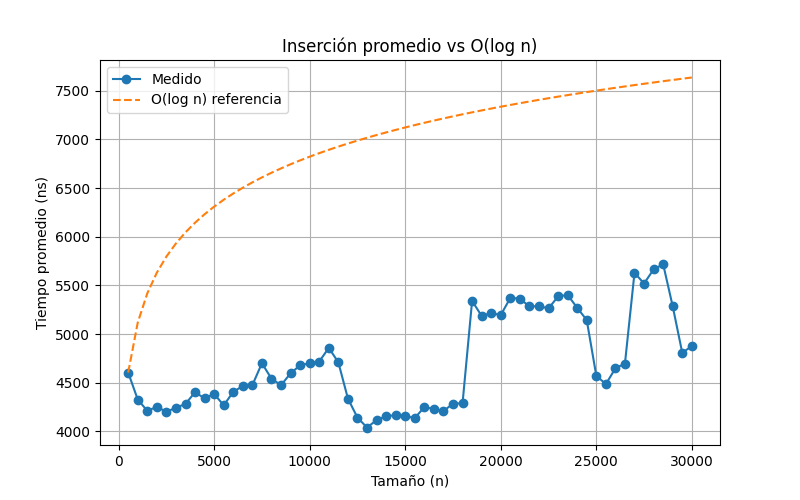
\includegraphics[width=0.9\columnwidth]{insert.png}
    \caption{Tiempo promedio de inserción vs tamaño de entrada.}
    \label{fig:insert_performance}
\end{figure}

La Figura~\ref{fig:insert_performance} muestra el comportamiento de la operación de inserción. Se observa que el tiempo de inserción crece de manera logarítmica con el tamaño de la entrada, confirmando la complejidad teórica de $O(\log n)$. Las variaciones menores en los tiempos son esperadas debido a la naturaleza de las rotaciones y recoloreos necesarios para mantener las propiedades del árbol.

\begin{figure}[H]
    \centering
    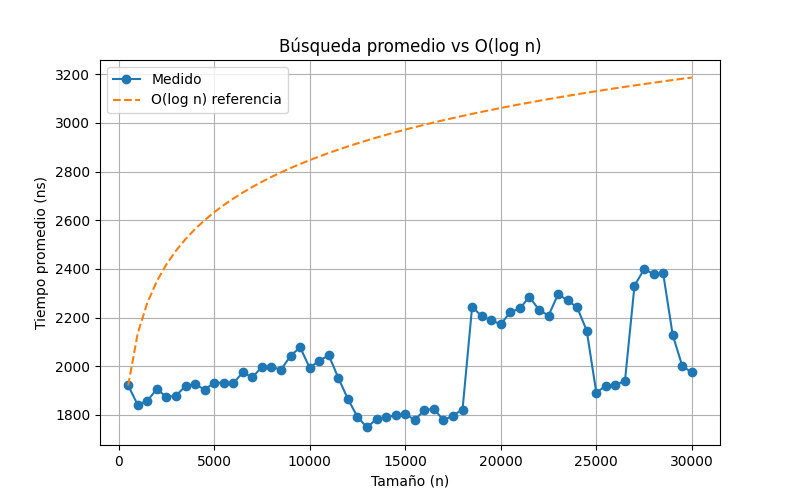
\includegraphics[width=0.9\columnwidth]{search.png}
    \caption{Tiempo promedio de búsqueda vs tamaño de entrada.}
    \label{fig:search_performance}
\end{figure}

En la Figura~\ref{fig:search_performance} se presenta el rendimiento de la operación de búsqueda. Los resultados demuestran una complejidad logarítmica consistente, con tiempos que se mantienen relativamente estables a medida que aumenta el tamaño del árbol. Esto confirma la eficiencia de la estructura balanceada del Red-Black Tree para operaciones de consulta.

\begin{figure}[H]
    \centering
    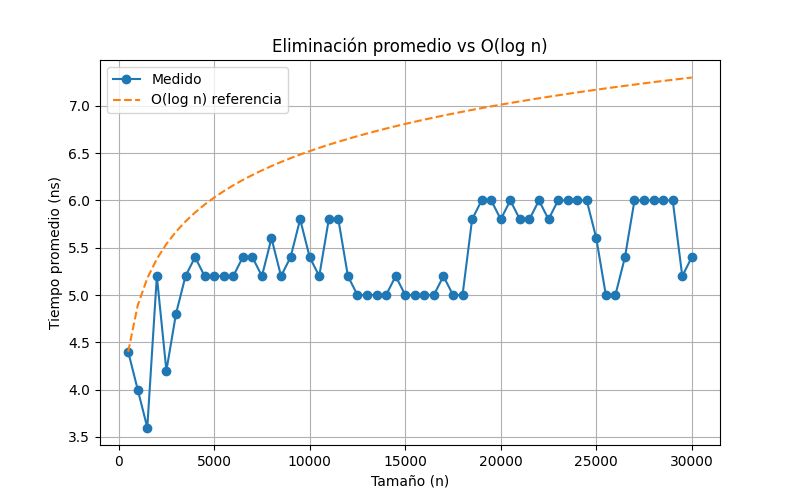
\includegraphics[width=0.9\columnwidth]{remove.png}
    \caption{Tiempo promedio de eliminación vs tamaño de entrada.}
    \label{fig:remove_performance}
\end{figure}

La Figura~\ref{fig:remove_performance} ilustra el comportamiento de la operación de eliminación. Aunque presenta mayor variabilidad que las operaciones anteriores, mantiene la complejidad logarítmica esperada. La variabilidad se debe a los diferentes casos que pueden ocurrir durante la eliminación (nodos con 0, 1 o 2 hijos) y las subsecuentes operaciones de rebalanceo.

\begin{figure}[H]
    \centering
    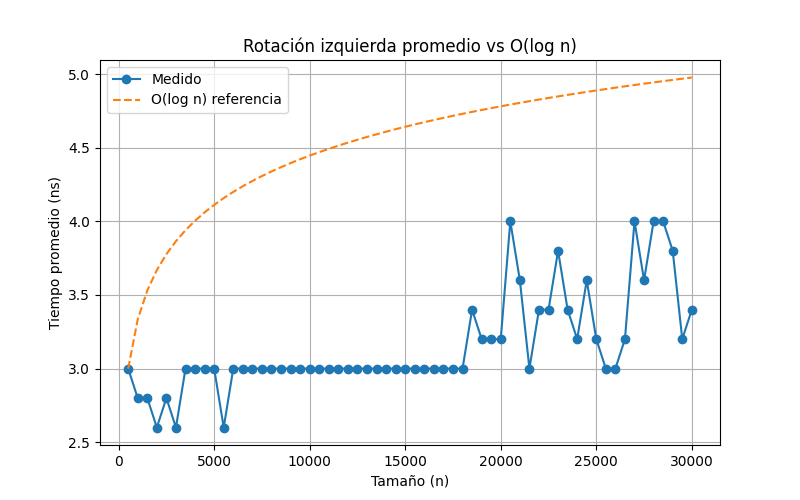
\includegraphics[width=0.9\columnwidth]{left_rotate.png}
    \caption{Tiempo promedio de rotación izquierda vs tamaño de entrada.}
    \label{fig:left_rotate_performance}
\end{figure}

\begin{figure}[H]
    \centering
    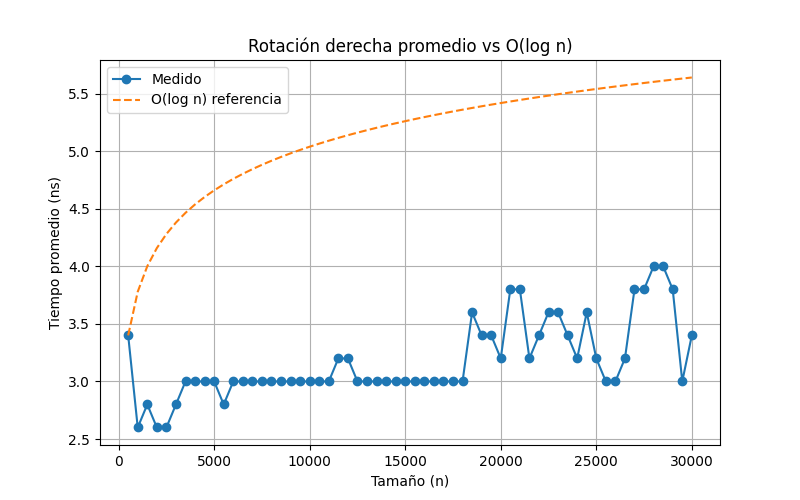
\includegraphics[width=0.9\columnwidth]{right_rotate.png}
    \caption{Tiempo promedio de rotación derecha vs tamaño de entrada.}
    \label{fig:right_rotate_performance}
\end{figure}

Las Figuras~\ref{fig:left_rotate_performance} y~\ref{fig:right_rotate_performance} muestran el rendimiento de las operaciones de rotación. Como era esperado, estas operaciones mantienen un tiempo constante $O(1)$ independientemente del tamaño del árbol, confirmando que las rotaciones son operaciones locales que solo afectan un número fijo de nodos. Los tiempos extremadamente bajos (del orden de nanosegundos) demuestran la eficiencia de estas operaciones fundamentales.



% Aquí puedes agregar un resumen de los resultados y observaciones finales.


% Fin Comparativa ---------------------------------------------------


% Ejemplos ---------------------------------------------------
%\vfill\eject
\section{Aplicaciones de los Árboles Rojo-Negro}

\subsection*{1. Implementación de Mapas y Conjuntos Ordenados}

En muchas bibliotecas estándar de lenguajes de programación, los Árboles Rojo-Negro son la base para estructuras como mapas y conjuntos que requieren orden.  
Por ejemplo, en \textbf{C++}, las estructuras \texttt{std::map} y \texttt{std::set} utilizan internamente Árboles Rojo-Negro. Estas permiten almacenar claves ordenadas en un mapa, o elementos únicos en un conjunto, manteniendo siempre el orden y permitiendo operaciones de búsqueda, inserción y eliminación en tiempo logarítmico \(O(\log n)\), incluso en el peor escenario. Esta eficiencia resulta clave en tareas como la creación de índices alfabéticos de palabras en un texto, donde el orden y el acceso rápido son esenciales.

De forma análoga, en \textbf{Java}, estructuras como \texttt{TreeMap} y \texttt{TreeSet} cumplen la misma función. Si, por ejemplo, se gestionan registros de usuarios ordenados por ID, \texttt{TreeMap} permite operar sobre ellos eficientemente, garantizando que el orden se preserve automáticamente tras cada modificación.

\subsection*{2. Gestión de Memoria y Procesos en Sistemas Operativos}

A nivel de sistemas, los Árboles Rojo-Negro son indispensables en operaciones críticas donde se requiere eficiencia y predictibilidad.  
Un ejemplo concreto es el \textbf{kernel de Linux}, que emplea estos árboles para gestionar las áreas de memoria virtual (VMAs) de los procesos. Cuando un proceso solicita memoria, el sistema necesita localizar rápidamente qué bloques están disponibles o ya en uso. La estructura balanceada de los Árboles Rojo-Negro permite hacer estas búsquedas de forma eficiente. También se usan en otras áreas del kernel, como la planificación de procesos (scheduling) o el manejo de estructuras de red.

Incluso en funciones tan fundamentales como la asignación y liberación de memoria —como las implementaciones de \texttt{malloc} y \texttt{free}—, algunos asignadores utilizan Árboles Rojo-Negro para llevar el control de los bloques de memoria libres, facilitando así una gestión eficiente del heap.

\subsection*{3. Bases de Datos e Indexación}

En bases de datos, donde el tiempo de respuesta en consultas es esencial, los Árboles Rojo-Negro también encuentran aplicación.  
Aunque las estructuras más comunes para índices en disco suelen ser los \textbf{Árboles B} o \textbf{B+}, los Árboles Rojo-Negro son una excelente opción para \textbf{índices en memoria}, especialmente en sistemas donde la estructura de datos completa cabe en RAM. Su rendimiento consistente en \(O(\log n)\) permite búsquedas rápidas incluso sobre grandes volúmenes de datos, manteniéndolos ordenados sin penalizar el tiempo de acceso.

\subsection*{4. Algoritmos de Red y Routers}

En el ámbito de las redes, la eficiencia en la búsqueda y el mantenimiento del orden es también un factor clave.  
En ciertos escenarios, los \textbf{routers} pueden utilizar estructuras basadas en árboles —incluyendo Árboles Rojo-Negro— para implementar \textbf{tablas de enrutamiento}. Estas permiten determinar rutas de forma rápida, lo cual es esencial para asegurar el flujo constante y eficiente de datos a través de la red.

\subsection*{5. Gráficos y Procesamiento de Imágenes}

Aunque menos frecuentes, los Árboles Rojo-Negro también tienen presencia en áreas como los gráficos computacionales.  
En algunos algoritmos de geometría computacional, utilizados para el procesamiento de gráficos o imágenes, puede ser útil contar con estructuras que organicen objetos —como puntos o segmentos— de forma eficiente. En estos casos, los Árboles Rojo-Negro pueden facilitar \textbf{búsquedas por coordenadas}, gracias a su capacidad de mantener datos ordenados y actualizables en tiempo logarítmico.


% Fin Ejemplos ---------------------------------------------------


% Conclusiones ---------------------------------------------------
\section{Conclusiones}
En conclusión, los árboles rojo-negro representan una solución eficiente y elegantemente diseñada para el manejo de datos ordenados. A diferencia de los árboles binarios de búsqueda tradicionales, que pueden volverse ineficientes al desbalancearse, los Red-Black Trees mantienen su estructura equilibrada de forma automática. Esto se logra mediante un sistema de coloración en donde cada nodo es rojo o negro en el cual impone ciertas reglas estructurales que aseguran que la altura del árbol se mantenga dentro de límites logarítmicos. Como resultado, operaciones fundamentales como la búsqueda, la inserción o la eliminación se realizan consistentemente en tiempo O(log n), incluso en los peores casos. Lo más destacable es que este equilibrio se logra a través de rotaciones y recoloreos, operaciones locales y de bajo costo (O(1)), que permiten al árbol adaptarse dinámicamente sin sacrificar rendimiento. Esta capacidad de autorregulación convierte a los árboles rojo-negro en una herramienta sumamente confiable y versátil para aplicaciones que requieren una gestión eficiente de datos, como diccionarios, bases de datos o sistemas de archivos.



% Fin Conclusiones ---------------------------------------------------


% Referencias ---------------------------------------------------


% FIN CONCLUSIONES --------------------




% REFERENCIAS BIBLIOGRAFICAS EJEMPLOS ---------------------
\begin{thebibliography}{00}

    \bibitem{baeldungRedBlack}
    M. Krimgen, ``Introduction to Red-Black Trees,'' \textit{Baeldung on Computer Science}. [Online]. Available: \url{https://www.baeldung.com/cs/red-black-trees}

    \bibitem{ahuja2021}
    H. Ahuja, ``Red-Black Tree. Introduction, Properties, Operations,'' \textit{Medium}, Apr. 13, 2021. [Online]. Available: \url{https://hardikahuja99.medium.com/red-black-tree-8cf904034a90}

    \bibitem{mushiba2024redblack}
    A. N. Mushiba, ``Red-Black Trees: An Essential Tool for Efficient Data Structures and Algorithms,'' \textit{ResearchGate}, Jan. 2024. [Online]. Available: \url{https://www.researchgate.net/publication/377471721}

    \bibitem{morin2013ods} 
    P. Morin, \textit{Open Data Structures}. Athabasca, AB, Canada: Athabasca University Press, 2013. [Online]. Available: \url{https://www.aupress.ca/app/uploads/120226_99Z_Morin_2013-Open_Data_Structures.pdf}

    \bibitem{linuxrbtree}
    R. Landley, ``Red-black Trees (rbtree) in Linux,'' \textit{The Linux Kernel Documentation}, Jan. 18, 2007. [Online]. Available: \url{https://docs.kernel.org/core-api/rbtree.html}
    
    \bibitem{jaiswal2018}
    D. Jaiswal, B. R., S. T. N., y K. K. S., ``Red-Black Tree \& Its Application,'' \textit{International Journal for Scientific Research \& Development}, vol. 6, no. 9, pp. 1–4, 2018. [En línea]. Disponible en: \url{https://www.ijsrd.com/articles/IJSRDV6I90249.pdf}

    \bibitem{cormen2001}
    T. H. Cormen, C. E. Leiserson, R. L. Rivest, and C. Stein, \textit{Introduction to Algorithms}, 2nd~ed. Cambridge, MA: The MIT Press, 2001.

    \bibitem{nguyen2019}
    H. M. Nguyen, ``Formal verification of a red-black tree data structure,'' MSc thesis, Dept. of Electrical Engineering, Mathematics and Computer Science, Univ. of Twente, Enschede, The Netherlands, Mar. 2019. [Online]. Available: \url{https://essay.utwente.nl/77569/1/Nguyen_MA_EEMCS.pdf}
    

\end{thebibliography}



\end{document}
